\documentclass[10pt,twocolumn,letterpaper]{article}

\usepackage{cvpr}
\usepackage[utf8]{inputenc}
\usepackage[T1]{fontenc}
\usepackage{gensymb}
\usepackage{graphicx}
\usepackage{caption}
\usepackage{subcaption}
\usepackage{mathtools}
\graphicspath{ {report3-imgs/} }
\usepackage{float}
\PassOptionsToPackage{hyphens}{url}\usepackage{hyperref}
\usepackage{minted}
\usemintedstyle{vs}

\cvprfinalcopy
\def\cvprPaperID{a1700831}


% begin of document
\begin{document}
\title{Assignment 3 - Method for Generating Image Descriptions}
\author{Yuanzhong Xia\\
University of Adelaide\\
SA, Australia\\
{\tt\small a1700831@student.adelaide.edu.au}
}
\maketitle

% abstract
\begin{abstract}
This report first introduces the problem: generating image descriptions (also named in image captioning), and its applications.
Previous approaches and their limitations are mentioned as well.
Then, the algorithm process from the original paper is discussed in three parts:
training, predicting and evaluating.
Next, my hypothesises, relative proofs and the limitations of proposed methods are discussed.
The reports also covers the experiments I did, and the experiments for verifying my hypothesises.
At last, there is a conclusion of what I learnt from this assignment, and the extensions that I can come out.
\end{abstract}

% content
\section{The Problem}
The problem is to give a description sentence in natural language for an input image.

This problem is very typical, because it is very challenging that it transforms information from ``image'' type to ``text'' type.
The input image should firstly be understood by the artificial intelligence,
then it should be able to output a descriptive text to tell what the input image shows.

The relative applications can be various, like: helping human to automatically pointing out the objectives
and events among a massive number of images, and helping visually impaired people to see.
But the most difficult challenge is not only understanding both image and natural language,
but also transforming the information from one type to another type.


\section{Background}
Before the original paper by Karpathy \textit{et al.} \cite{origin}. There are plenty of researches challenging this problem,
which can be mainly divided into three types.

\subsection{Image annotating strategy}
A typical way to annotate images is classifying or tagging images \cite{everingham}, \cite{russakovsky}.
In a fixed word dictionary, the image tagging can be more meaningful because unwanted words are discarded at the beginning.
The weakness is that the words in dictionary are often not rich enough.

Barnard \textit{et al.} \cite{barnard} and Socher \textit{et al.} \cite{socher}'s researches uses the images,
whose segments are annotated instead the whole image, as the training input data.
That helps the object recognition process, but requires more human works.

Gould \textit{et al.}'s research \cite {gould} used a method to extract scene feature,
so that the relationships between objects and the scene can be easily connected.
However, their work was focusing on labelling the scene, while the proposed method is used to
generate richer and high-level descriptions of the image, no matter what the scene labels are.


\subsection{Description generating strategy}
Methods from Kulkarni \textit{et al.} \cite{kulkarni} limit the resulting sentence number in one;
whereas the original paper's authors think that manual restriction is not necessary and it reduces the artificial intelligence's creativity.

Matuszek \textit{et al.} \cite{matuszek} used grounding dependency tree relations which arrange words in a vector space.
The vector space would limit the results to some extend, like the resulting sentence length, etc.


\subsection{Connecting between images and natural language strategy}
The earlier pioneering methods by Farhadi \textit{et al.} \cite{farhadi} hard-coded visual concepts and explicitly defined sentence.
Images objects or scenes are pre-defined, then marked images are learnt by the system so that the system can recognize defined things.
However, these methods limited the language variety and required much human works to define the connecting between language words and the images first.

Now, pre-trained image/word vectors are quite popular.
For images, ImageNet \cite{imagenet} is a very popular pre-trained image recognition model;
for words, previous works \cite{bengio}, \cite{socher2}, \cite{mikolov} mentioned the pre-trained word vectors
to obtain low-dimensional representations of words.
Additionally, in the original paper, the authors use these pre-trained models as well.


\section{Algorithm Description}
Unlike the previous approaches, the proposed method in Karpathy \textit{et al.}'s paper is to make the artificial neural networks
learn the pattern between images and sentences automatically.
Therefore, there is no limitation for this method literally,
because the training data can be arbitrary, and the model thus will be adjusted by the training data.

\subsection{Training}
The overview of training steps is as follows,
\begin{enumerate}
    \item Prepare the training images and corresponding sentences;
          \textit{(datasets mentioned in the paper are flickr8k, flickr30k and MSCOCO,
          and sometimes each image has multiple descriptive sentences.)}
    \item Extract 4096 dimensional features vector using pre-trained CNN model on ImageNet \cite{imagenet};
          \textit{(this model contains objects of 200 classes, which is described in ImageNet Detection Challenge \cite{inch}.)}
    \item Train the multimodal RNN sentence generator which takes a word to predict the next following word, by passing the words one by one and the image feature matrix;
          \textit{(``START'' and ``END'' are two special tokens in this RNN, and the words are sent to the RNN one by one.)}
\end{enumerate}

\subsection{Predicting}
To predict an image using existing model:
\begin{enumerate}
    \item Prepare testing images and prediction RNN model;
    \item Extract 4096 dimensional feature vector using pre-trained CNN model on ImageNet;
          \textit{(same as training.)}
    \item Generate description from multimodal RNN by setting ``START'' token and image representation matrix;
          \textit{(until ``END'' is generated, the description is finished generating.)}
\end{enumerate}

\subsection{Benchmark}
The original paper also mentions the methods for predicting region text information (to mark the regions like Figure \ref{fig:region}):
\begin{enumerate}
    \item When having the image's feature vector;
    \item Calculate the image representation matrix using top 19 detected known objects by the dot product between feature vector and a parameter matrix $W_{m}$;
          \textit{(the representation matrix in the paper is in the shape of 20 $h$-dimensional vectors, thus this is the recognizable resolution.)}
    \item Calculate the sentence representation vector using Bidirectional Recurrent Neural Network (BRNN) \cite{brnn};
          \textit{(each input sentence sequence is transformed into a $h$ dimensional vector;
          during the calculation, BRNN takes two directional word relations to maintain a context;
          then, a word vocabulary is built automatically by the methods from Mikolov et al. \cite{mikolov}.)}
    \item Calculate image-sentence score by dot product between sentence representation vector and image representation matrix and a $max$ operation;
          \textit{(this method is proved by their previous work \cite{karpathy},
          and the resulting image-sentence score is actually calculated by the image region-word score,
          with the dimension of 20.)}
    \item Align words with corresponding regions in Markov Random Field (MRF) to get an annotated region set;
          \textit{(each region has multiple words aligned with;
          to find the best alignment, the authors use dynamic programming by Viterbi et al. \cite{viterbi}.)}
\end{enumerate}

The ``image-sentence score'' is the benchmark value.
Experiments from the original paper use this score ranking for comparisons.

\begin{figure*}
    \begin{center}
        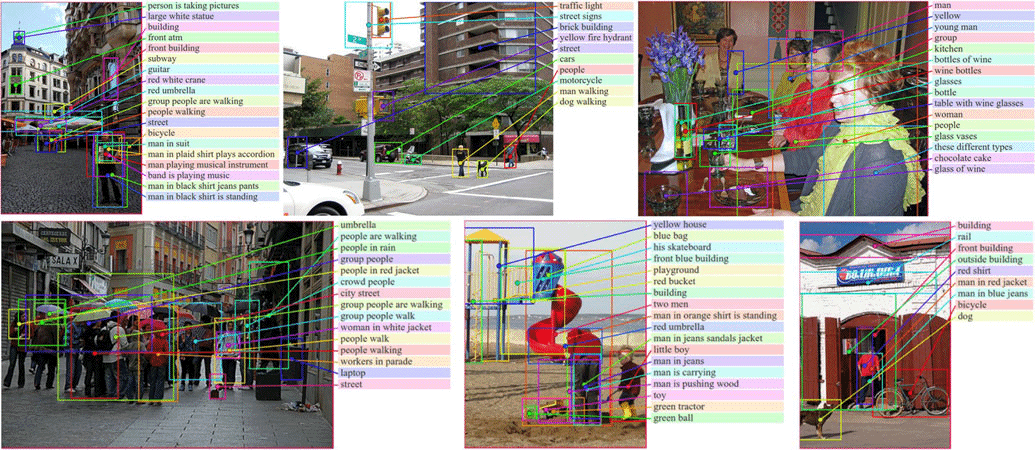
\includegraphics[width=0.9\textwidth]{region.png}
    \end{center}
    \caption{The region prediction from the original paper. This figure is the Fig. 9 in original paper.}
    \label{fig:region}
\end{figure*}


\section{Hypothesis and limitations} \label{sec:hl}
\subsection{Two model issue}
The proposed methods in original paper use two models for the final prediction:
the object recognition model and description generator model.
Two models are trained with different datasets.

Thus, my hypothesis is,
\begin{enumerate}
    \item the objects which are in the first training dataset but not in the second dataset
          will take an unnecessary weight in the first model;
    \item the objects which are not in the first training dataset but in the second dataset
          will not be detected.
\end{enumerate}

In the original paper, the first model is pre-trained for object recognition by ImageNet \cite{imagenet}.
This is a tree-based model (database) containing 5247 categories of objects, and built by around 50 million images.
And the original paper uses 200 categories from The ImageNet Detection Challenge \cite{inch}.
Given the input image, the nearest neighbour methods can vote and return the recognized object.
However, plenty of tree nodes are taken by unused objects, thus the the rate of mis-recognition increases, which supports my first statement.

For the second statement, the image representation matrix is calculated as
$$v = W_{m} \left [ CNN_{\theta_{c}}(I_{b}) \right ] + b_{m}$$
the resulting matrix from $CNN$ will have un-detected cells filling with $0$.
And therefore, after the dot product with sentence representation vector
$$S_{kl} = \sum_{t \in texts} max_{i \in cells}(v_{i}^{T}s_{t})$$
where $v_{i}^{T}$ is the image representation matrix and $s_{t}$ is the representation matrix.
The un-detected words will thus result in $0$.
Hence, those objects not in the recognition model (first dataset) cannot be detected even if they are in the second dataset.


\subsection{Resolution issue}
The image feature size is fixed to 4096 dimensions in the original paper.
My hypothesis is that, if the image is far too larger than its inside objects, the objects cannot be recognized,
even if the objects are very clear when zooming in the image.

In the original paper, the feature set of an image is expressed in a 4096 dimensional vector.
If the image is super large, and the objects cannot be effectively detected and stored in the feature vector,
the image will be difficult to be summarized correctly. An experiment is mentioned in Section \ref{sec:hs}.


\subsection{Unexpected object issue}
My hypothesis is that unexpected objects will result in unexpected sentences.

This is a common machine learning issue, but with different appearance on results.
I guess the results will still be a complete sentence, even when there is nothing in the input image,
because the structure of RNN is building sentence from the beginning to the end.
The experiment is discussed in Section \ref{sec:uo}.


\subsection{Language grammar issue}
% The proposed methods in original paper use word2vec to group the words \cite{mikolov},
% which helps the model to distinguish coordinate components or other grammatical relationships,
% e.g. ``A and B'' is equal to ``B and A''.

My hypothesis is that, although it learns from non-systematic sentences,
there should still seldom be grammar errors because the use of contexts.

% TODO: how to tag more effectively (+5 times selected)
Due to the RNN training process in the original paper, predicting each next word requires a context,
which helps forming the grammatically correct sentence.
An experiment on this hypothesis is mentioned in Section \ref{sec:lg}.


\subsection{Resulting number issue} \label{sec:rni}
My hypothesis is that the proposed methods cannot distinguish the correct number in most times.

Although the training input word sequence has been been grouped by word2vec,
the words representing numbers are not treated separately in proposed methods,
i.e. all sentence components are treated equally in RNN.
That means the word ``two'' in ``two men'' and ``two women'' are treated separately,
When current word is ``two'', the next possible words are ``men'' and ``women''.

However, if the training data contains ``two men'' and ``a woman'' only,
the resulting sentence is impossible to contain ``two women'' and ``a man'',
because ``two'' is followed by ``men'', ``a'' is followed by ``woman'',
and there is no change that ``two'' is followed by neither ``woman'' nor ``women''.
An experiment on this hypothesis is shown in Section \ref{sec:rn}.


\section{Experiments}
The experiments are based on the authors' codes \footnote{\url{https://github.com/karpathy/neuraltalk}} and pre-trained model
\footnote{\url{http://cs.stanford.edu/people/karpathy/neuraltalk/}} on Flickr8k dataset.
The image recoginision pre-trained model is a ``caffe'' ported model \footnote{\url{http://www.robots.ox.ac.uk/~vgg/research/very_deep/}}, based on ImageNet.
The RNN structure is as same as described in the original paper.

The experiments are devided into two types:
\begin{enumerate}
    \item Recall test: the model is tested on training data;
    \item Fresh test: the model is tested on new data;
\end{enumerate}

My metric test benchmark functions are defined as:
$$B = max(\frac{1}{2}P(CorrectWord) + \frac{1}{2}P(CorrectOrder)$$
where the word correction rates of the resuling sentence $P(CorrectWord)$ is calculated by:
$$P(CorrectWord) = \frac{num}{average(length)}$$
where $num$ is the number of words that exists in both correct sentences and the resulting sentence.
The probability of words appearing in correct order $P(CorrectOrder)$ is calculated by:
$$P(CorrectOrder) = \frac{LCSLength}{average(length)}$$
where LCS means the longest common subsequence, which is a very classical dynamic programming problem.
Here is an example:
\begin{itemize}
    \item Input A: ['a', 'brown', 'dog', 'is', 'running', 'through', 'the', 'grass']
    \item Input B: ['a', 'brown', 'dog', 'is', 'running', 'outside']
    \item LCS: ['a', 'brown', 'dog', 'is', 'running']
\end{itemize}

\subsection{Recall test}
For the recall test, I randomly selected 1,000 images from Flickr8k dataset using
``shuf -zen1000 f8k\_data/\text{*} | xargs -0 mv -t neuraltalk/rf1kfrom8k/'' commands.

Then, extract features and do the testing. The testing results are shown in Table \ref{tab:recall}.
And detailed results are in web submission ``benchmark'' folder.

The best predictiong details are:
\begin{itemize}
    \item Training: ['a', 'dog', 'runs', 'through', 'the', 'grass']
    \item Predicting: ['a', 'dog', 'runs', 'through', 'the', 'grass']
    \item Interset: ['a', 'dog', 'runs', 'through', 'the', 'grass']
\end{itemize}

The worst prediction details are:
\begin{itemize}
    \item Training: ['two', 'dogs', 'are', 'playing', 'together']
    \item Predicting: ['a', 'black', 'dog', 'bites', 'a', 'white', 'dog', 'on', 'the', 'grass']
    \item Interset: []
\end{itemize}

\begin{table}[]
\centering
\begin{tabular}{ccc}
\hline
max    & min    & average \\ \hline
1.0000 & 0.0000 & 0.4238  \\ \hline
\end{tabular}
\caption{Recall testing results.}
\label{tab:recall}
\end{table}

\subsection{Fresh test}
For the first fresh test, I randomly selected 1,000 images from Flickr30k dataset,
and use the model trained from Flickr8k dataset.

Then, extract features and do the testing using the same model. The final results are shown in Table \ref{tab:fresh1}.

The best prediction details are:
\begin{itemize}
    \item Training: ['a', 'brown', 'dog', 'is', 'running', 'through', 'the', 'snow']
    \item Predicting: ['the', 'brown', 'dog', 'is', 'running', 'through', 'the', 'snow']
    \item Intersection: ['brown', 'dog', 'is', 'running', 'through', 'the', 'snow']
\end{itemize}

The worst prediction details are:
\begin{itemize}
    \item Training: ['a', 'man', 'in', 'a', 'red', 'jacket', 'is', 'standing', 'in', 'front', 'of', 'a', 'building']
    \item Predicting: ['people', 'are', 'boarding', 'an', 'almost-full', 'public', 'bus', 'in', 'brazil']
    \item Intersection: ['in']
\end{itemize}

\end{itemize}
\begin{table}[]
\centering
\begin{tabular}{ccc}
\hline
max    & min    & average \\ \hline
0.9042 & 0.0981 & 0.3745  \\ \hline
\end{tabular}
\caption{Fresh testing results on 30k dataset, by 8k model.}
\label{tab:fresh1}
\end{table}

Another fresh test is using a model trained by MSCOCO dataset to test 1,000 images from Flickr8k.
The final results are in Table \ref{tab:fresh2}.

The best prediction details are:
\begin{itemize}
    \item Training: ['a', 'young', 'boy', 'is', 'sitting', 'on', 'a', 'toilet']
    \item Predicting: ['a', 'young', 'boy', 'sitting', 'on', 'a', 'blue', 'toilet']
    \item Intersection: ['a', 'young', 'boy', 'sitting', 'on', 'a', 'toilet']
\end{itemize}

The worst prediction details are:
\begin{itemize}
    \item Training: ['a', 'group', 'of', 'people', 'standing', 'around', 'a', 'table', 'with', 'a', 'cake']
    \item Predicting: ['several', 'women', 'wearing', 'pink', 'energizer', bunny', 'ears', 'point', 'to', 'the', 'right']
    \item Intersection: []
\end{itemize}

\begin{table}[]
\centering
\begin{tabular}{ccc}
\hline
max    & min    & average \\ \hline
0.8661 & 0.0000 & 0.3616  \\ \hline
\end{tabular}
\caption{Fresh testing results on 8k dataset, by MSCOCO model.}
\label{tab:fresh2}
\end{table}


\subsection{Experiments for hypothesis}
\subsubsection{High resolution experiment} \label{sec:hs}
To verify my hypothesis, I firstly tested an image with the Flickr8k model, whose result is shown in Figure \ref{fig:hsori}.
Then, I expanded the background of the image without any zooming, and the result can be seen in Figure \ref{fig:hs}.

That proved my hypothesis was correct because the model did not know what was on that image.
It can also be proved in Section \ref{sec:ui} that ``a man'' is the default result in this case.

\begin{figure}[t]
    \begin{center}
        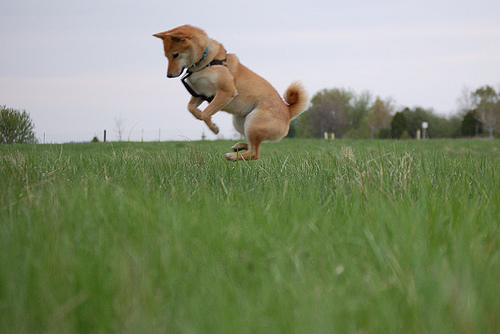
\includegraphics[width=0.9\linewidth]{2584487952_f70e5aa9bf_ori.jpg}
    \end{center}
    \caption{A picture with resulting sentence of ``a brown dog is running through the grass''.}
    \label{fig:hsori}
\end{figure}

\begin{figure}[t]
    \begin{center}
        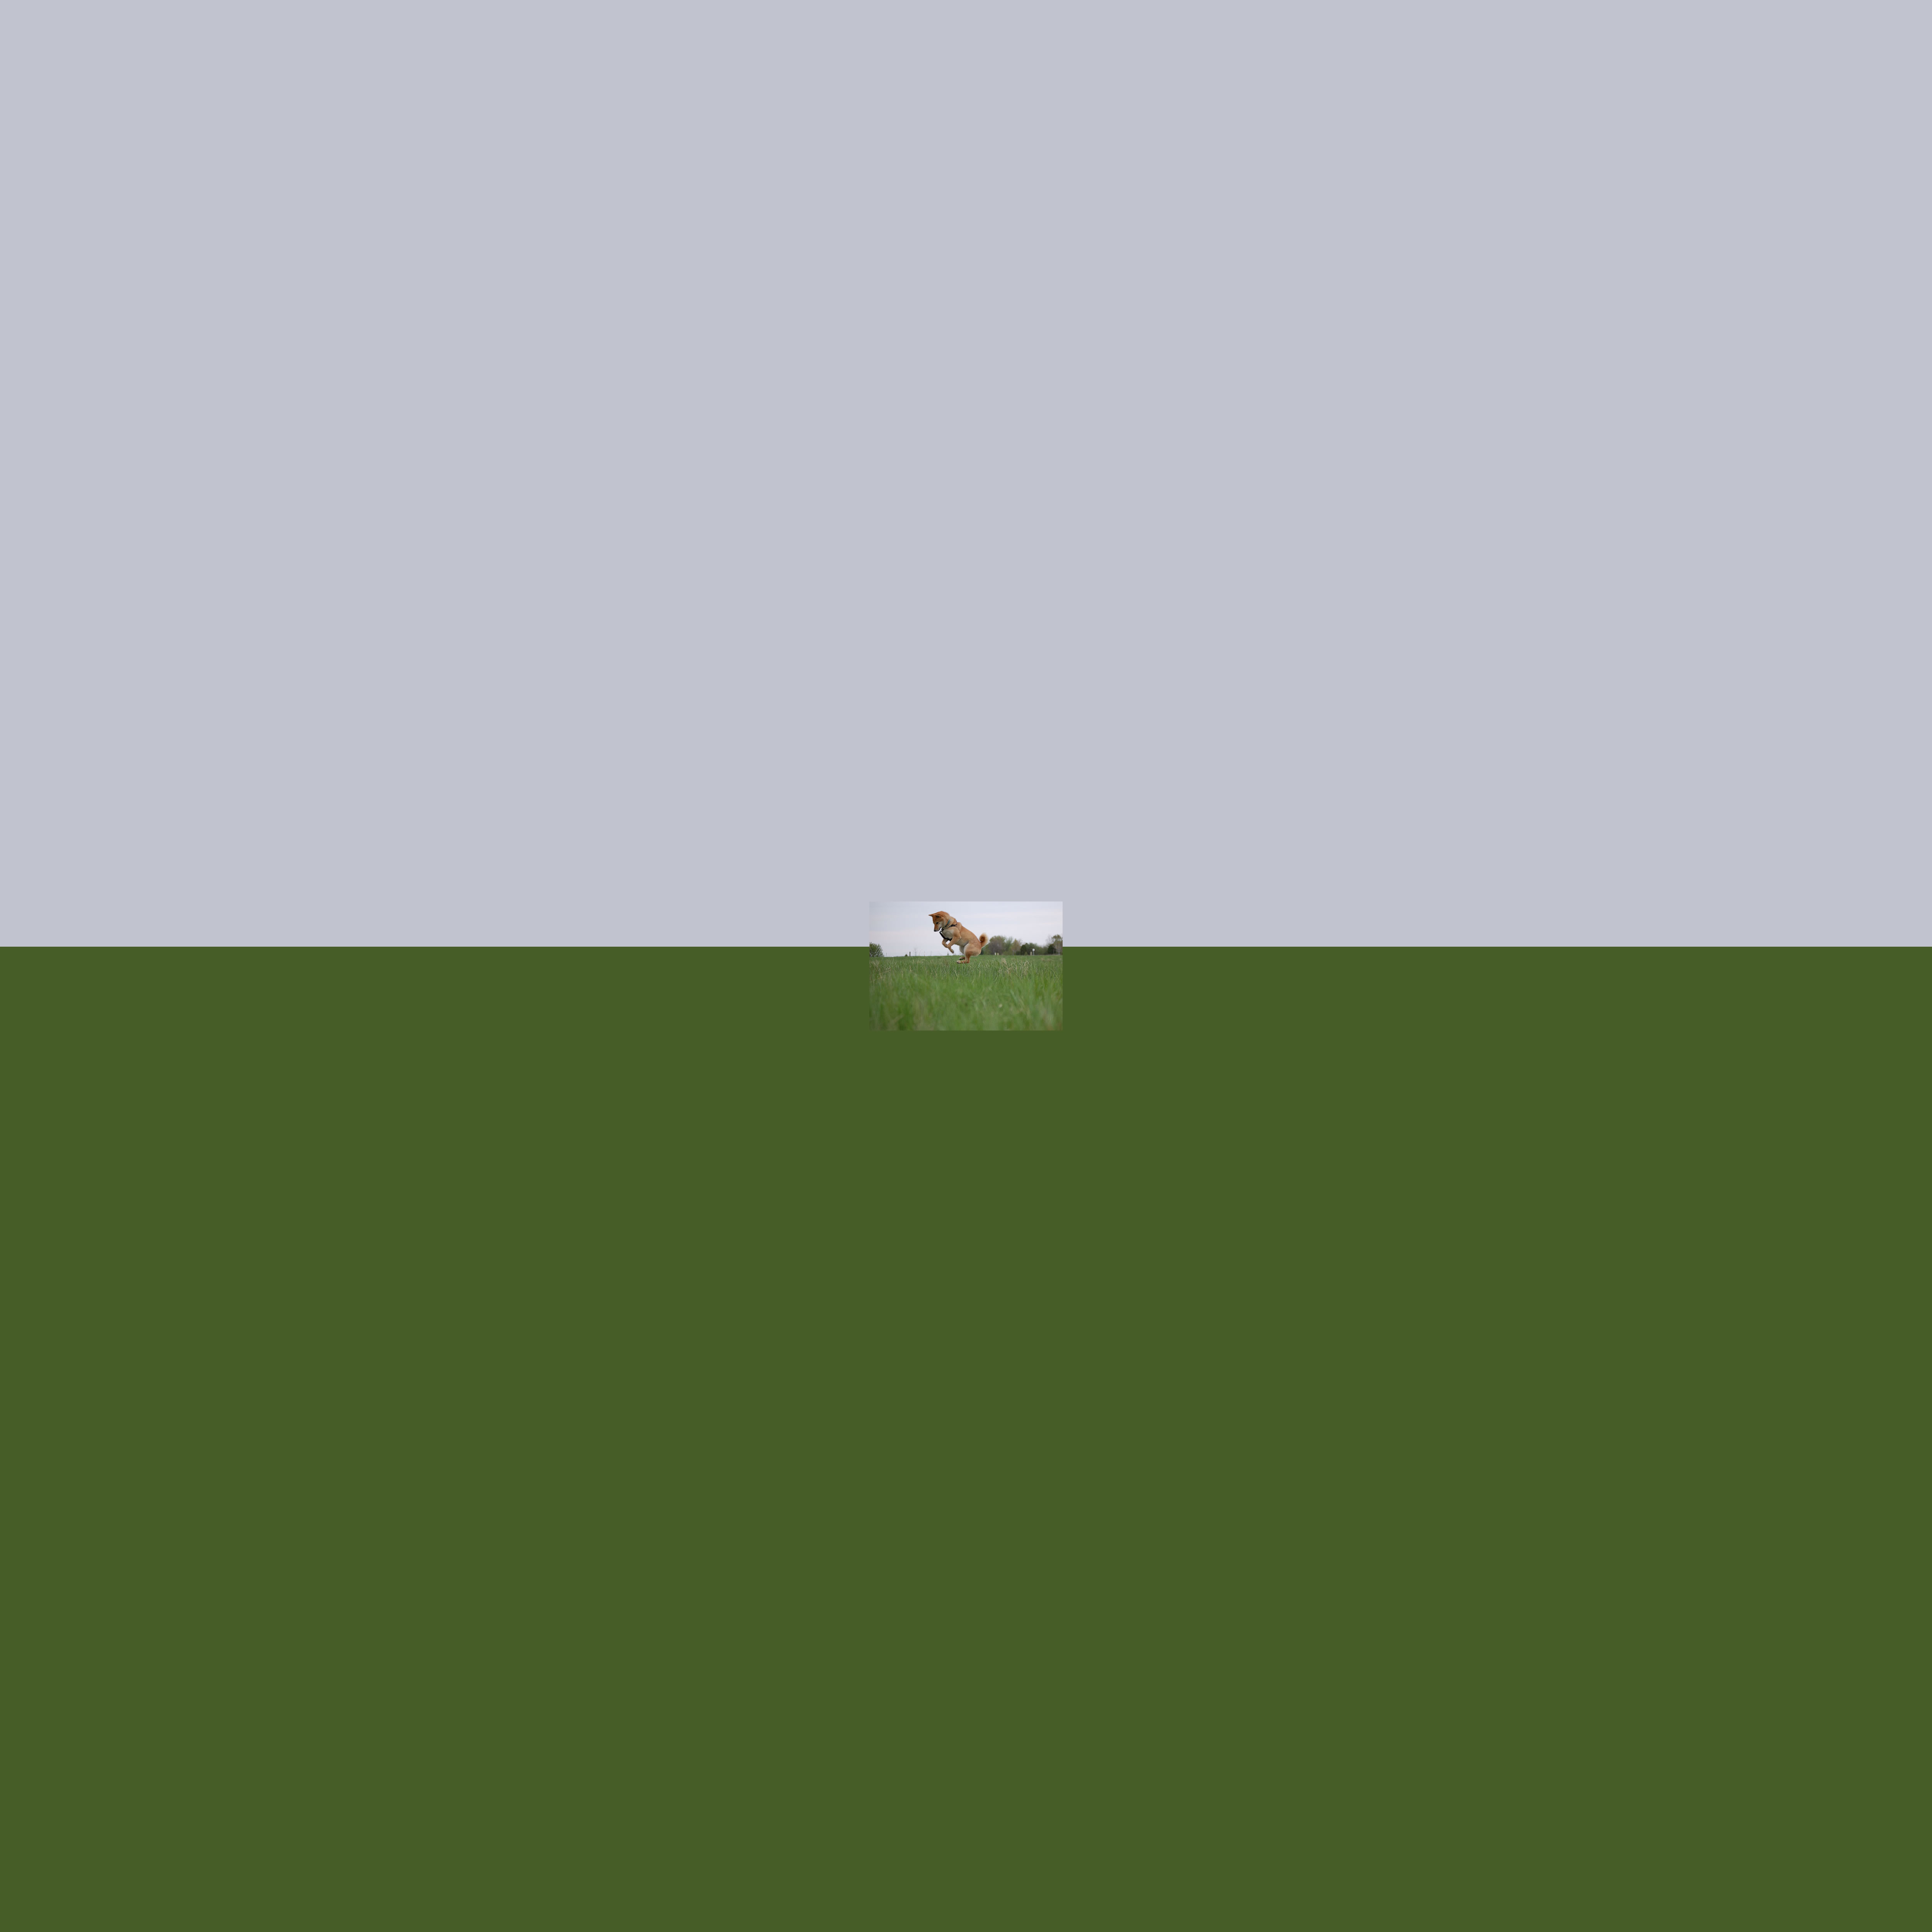
\includegraphics[width=0.9\linewidth]{2584487952_f70e5aa9bf.jpg}
    \end{center}
    \caption{A $5000 \times 5000$ px picture, with a dog in the center, the resulting sentence is ``a man is rock climbing''.}
    \label{fig:hs}
\end{figure}

\subsubsection{Unexpected object experiment} \label{sec:uo}
To test this hypothesis, I put a pure green image into the prediction model.
And the result is shown in Figure \ref{fig:pure}.
This also proved that hypothesis that even there was nothing in the image, the model would still give out a complete sentence.

\begin{figure}[t]
    \begin{center}
        
\includegraphics[width=0.9\linewidth]{pure.jpg}
    \end{center}
    \caption{A $600 \times 450$pure green image with the resulting sentence of ``a man is jumping in the air''.}
    \label{fig:pure}
\end{figure}

\subsubsection{Language grammar experiment} \label{sec:lg}
To test this hypothesis, I selected 100 images from Flickr8k randomly, and tested them using the Flickr8k model.
The benchmark results are:
\begin{enumerate}
    \item Max: 0.8819
    \item Min: 0.1125
    \item Average: 0.4137
\end{enumerate}

By manual checking the 100 prediction sentences, only one sentence had obvious grammar error.
That sentence is ``a man and woman walk down a street''.
The use of ``a man and woman'' looks incorrect.
However, the interesting part is, this is an coincidence because a training data contains exact this usage:
in ``1198194316\_543cc7b945.jpg'', one of its training sentences is ``A man and woman standing in front of a refreshment stand''.

Looking out of grammar issue, the meaning can have problems.
Here is an example, one of the 100 prediction sentences is
``a man in a black shirt and a woman in a white shirt and a black shirt''.
``A man in a white shirt and a black shirt'' does not make sense.

Therefore, the grammar error rate is almost 0\%, but the meaning of resulting sentences can often be confusing.


\subsubsection{Resulting number experiment} \label{sec:rn}
Using the same prediction sentence results mentioned above, by manual checking.
At first, filter the images containing only one object, there are 7 images containing more than one objects,
but 4 of them have a wrong number of subjects. Two of them used a word ``plenty of'' to describe the number, which are counted as correct.

Therefore, the hypothesis is correct that the model from the original paper does not have the ability to count the numbers.


\section{Conclusion}
Through this assignment, I learnt the new research approaches: using existing databases/models directly.
It is surprising to see that the authors take the CNN from ImageNet directly
to achieve a high correctness rate for object recognitions.

Unlike what I thought before, learning an approach from a research paper,
and I have to follow the steps and try to recur the whole process.
Sometimes, the author does not publish the source codes and tools,
thus it is not easy to reuse the existing codes and outcomes, thus recurring the process is necessary.

However, in most cases, including this research, even the comments in the source codes from the authors say
that it is encouraged to build extensions based on their codes.
Moreover, this is what the authors did for the their paper, they applied the ImageNet database and model directly,
and text2vec tools by Mikolov \textit{et al.}, etc.
This helps reducing the work a lot, and motivate the research for more wonderful extensions.

Regarding the methods in this paper, it is very happy to see this method breaking out the sentence structure.
They use multimodal RNN for fully reasonable context training,
and can significantly make resulting sentences correct grammatically.
Although combining CNN and RNN together is a typical solution for image captioning,
they evolve a lot of extensions to make the results more accurate.

The potential limitations are mentioned in Section \ref{sec:hl}.
To overcome those limitations, increasing the training dataset is obviously a solution,
as the methods is universal, and highly depending on the training dataset.

Additionally, as I mentioned in Section \ref{sec:rni}, the number are not handled very well in this training methods.
I think, for example, numbers can be specially treated/learnt as another model.
Since the objects can be recognised, counting objects should not be a big issues if
the number model has already known how to describe the objects.


% Bibliography
\begin{thebibliography}{99}
\bibitem {origin}
A. Karpathy and L. Fei-Fei, Deep visual-semantic alignments for generating image descriptions,
In \textit{Proceedings of the IEEE Conference on Computer Vision and Pattern Recognition}, pp. 3128-3137, 2015.

\bibitem {kulkarni}
G. Kulkarni, et al., Baby talk: Understanding and generating simple image descriptions,
In \textit{Proc. IEEE Conf. Comput. Vis. Pattern Recog.}, pp. 1601-1608, 2011.

\bibitem {farhadi}
A. Farhadi, et al., Every picture tells a story: Generating sentences from images,
In \textit{Proc. 11th Eur. Conf. Comput. Vis.}, pp. 15-29, 2010.

\bibitem {everingham}
M. Everingham, L. Van Gool, C. K. I. Williams, J. Winn, and A. Zisserman, The Pascal visual object classes (VOC) challenge,
In \textit{Int. J. Comput. Vis.}, vol. 88, no. 2, pp. 303–338, 2010.

\bibitem {russakovsky}
O. Russakovsky, et al., Imagenet large scale visual recognition challenge,
In \textit{Int. J. Comput. Vis.}, vol. 115, no. 3, pp. 211–252, 2015.

\bibitem {barnard}
K. Barnard, P. Duygulu, D. Forsyth, N. De Freitas, D. M. Blei, and M. I. Jordan, Matching words and pictures,
In \textit{J. Mach. Learn. Res.}, vol. 3, pp. 1107–1135, 2003.

\bibitem {socher}
R. Socher and L. Fei-Fei, Connecting modalities: Semi-supervised segmentation and annotation of images using unaligned text corpora,
In \textit{Proc. IEEE Conf. Comput. Vis. Pattern Recog.}, pp. 966–973, 2010.

\bibitem {gould}
S. Gould, R. Fulton, and D. Koller, Decomposing a scene into geometric and semantically consistent regions,
In \textit{Proc. IEEE 12th Int. Conf. Comput. Vis.}, pp. 1–8, 2009.

\bibitem {matuszek}
C. Matuszek, N. FitzGerald, L. Zettlemoyer, L. Bo, and D. Fox, A joint model of language and perception for grounded attribute learning,
In \textit{Proc. 29th Int. Conf. Mach. Learn.}, pp. 1671–1678, 2012.

\bibitem {bengio}
Y. Bengio, H. Schwenk, J.-S. Senecal, F. Morin, and J.-L. Gauvain, Neural probabilistic language models,
In \textit{Innovations in Machine Learning. Berlin, Germany}, 2006.

\bibitem {socher2}
R. Socher, J. Pennington, and C. Manning, Glove: Global vectors for word representation,
In \textit{Proc. Empirical Methods Natural Language Process.}, pp. 1532–1543, 2014.

\bibitem {mikolov}
T. Mikolov, I. Sutskever, K. Chen, G. S. Corrado, and J. Dean, Distributed representations of words and phrases and their compositionality,
In \textit{Proc. Advances Neural Inf. Process. Syst.}, pp. 3111–3119, 2013.

\bibitem {imagenet}
J. Deng, W. Dong, R. Socher, L.-J. Li, K. Li, and L. Fei-Fei, ImageNet: A large-scale hierarchical image database,
In \textit{Proc. IEEE Conf. Comput. Vis. Pattern Recog.}, pp. 248–255, 2009.

\bibitem {inch}
O. Russakovsky, et al., Imagenet large scale visual recognition challenge,
In \textit{Int. J. Comput. Vis.}, vol. 115, no. 3, pp. 211–252, 2015.

\bibitem {brnn}
M. Schuster and K. K. Paliwal, Bidirectional recurrent neural networks,
In \textit{IEEE Trans. Signal Process.}, vol. 45, no. 11, pp. 2673–2681, 1997.

\bibitem {karpathy}
A. Karpathy, A. Joulin, and F. F. F. Li, Deep fragment embeddings for bidirectional image sentence mapping,
In \textit{Proc. Advances Neural Inf. Process. Syst.}, pp. 1889–1897, 2014.

\bibitem {viterbi}
A. J. Viterbi, Error bounds for convolutional codes and an asymptotically optimum decoding algorithm,
in \textit{IEEE Trans. Inf. Theory}, vol. TIT-13, no. 2, pp. 260–269, 1967.

\end{thebibliography}

\end{document}
